
\documentclass[a4paper, 12 pt]{IEEEtran}  
%\bibliographystyle{IEEEtran}      
\bibliographystyle{alpha}

%some formatting changes to move header and footer position manually to the right spot:
\usepackage{fancyhdr}
\renewcommand{\headrulewidth}{0pt}%potential line between header and body
\addtolength{\headheight}{1.2 cm}%more space for header
\addtolength{\headsep}{-.3 cm}%pull body up
\addtolength{\footskip}{-.5 cm}%pull footer up
%see the doc1ument https://tobi.oetiker.ch/lshort/lshort.pdf, page 115 for definition of main formatting variables

\usepackage{psfrag}%needed to replace text in figures with latex text. Note that this package does not work with pdfLaTeX, so make sure the compiler is set to "LaTeX".
\usepackage{amsmath,amssymb,amsfonts}%for equations
\usepackage{siunitx} %to use the correct spacing between number and unit. Replaces the older package "units"
  
                    
%some more useful packages:                     
\usepackage{dsfont,latexsym,cite, comment, graphicx,color}
\usepackage{url, hyperref}
\usepackage[T1]{fontenc}

%if you want to put several images into one figure:
\usepackage{subfigure}
\newcommand{\goodgap}{%for subfigure package
\hspace{\subfigtopskip}%
\hspace{\subfigbottomskip}}

%some commands to simplify math typing:
\newcommand{\V}[1]{\boldsymbol{#1}}%use this command for vectors
\newcommand{\M}[1]{\mathbf{#1}}%use this command for matrices
\DeclareMathOperator\sgn{sgn}%make sure that sign is interpreted as a function, not as a variable
\newcommand{\ud}{\mathrm{d}} 							% roman d for derivatives
\hyphenation{Re-ge-lungs-tech-nik}%Sometimes, default hyphenation is incorrect. Then, you have to specifiy it here. To find the right hyphenation, look at www.merriam-webster.com.

%Here, you may include other packages or provide new commands:
%Sprachpakete deutsch
\usepackage[ngerman]{babel}	%Neue Rechtschreibung

%Ueberschriften ändern !!! muss vor titlesec stehen!
%%\usepackage{sectsty}
%für extra schmale Abstände in Überschriften in den Übungsblätter:
%%\usepackage{titlesec}


\title{Mission Statement - Zielgruppe für einen Frauenstudiengang Elektrotechnik}
\author{Ann-Morla Meyer}
\date{January 2023}

\begin{document}

%%%%%%%%%%%%%%%%%%%%%%%%%%%%%%%%%%%
\fancyhf{} %clean header and footer
\fancyhead[L]{\sf \small Ann-Morla Meyer: Mission Statement- Zielgruppe für einen Frauenstudiengang Elektrotechnik, Berlin, Germany, \today} %header left
\fancyfoot[C]{\thepage} %footer centered
\maketitle
\thispagestyle{fancy}%to include the header on the first page
%\pagestyle{plain}%no header on the other pages
%%%%%%%%%%%%%%%%%%%%%%%%%%%%%%%%%%%%%%%%%%%%%%%%%%%%%%%%%
%AUFGABEN

%Spezielle Überschriftenformate im Übungsblatt
%\titlespacing{\section}{0pt}{*5}{*1}
%\titlespacing{\subsection}{0pt}{*0.5}{*-1}
%%%\sectionfont{\fontsize{13}{13}\selectfont}		
%%%\subsectionfont{\fontsize{11}{11}\selectfont}	
%\renewcommand{\thesubsection}{\arabic{section} \alph{subsection})}
%%%%%%%%%%%%%%%%%%%%%%%%%%%%%%%%%%%%%%%%%%%%%%%%%%%%%%%%%%%%%

\maketitle
%\tableofcontents

%Strobel:
%i) Unterscheidet sich das Lernen (insb. in MINT Fächern) grundsätzlich zwischen den Geschlechtern und lässt sich das wissenschaftlich belegen? Welche weiteren Faktoren spielen hier eine Rolle?
%ii) Gibt es Studien die erklären können, warum gerade Deutschland ein (subjektiv) großes Problem damit hat Mädchen für MINT Fächer / Frauen für Ingenieurs-/Naturwissenschaften zu begeistern?
%iii) Welche Lernformen/-inhhalte und Motivation sind besonders geeignet weibliche Personen für Ingenieursfächer zu begeistern (im Gegensatz zu ihren männlichen Kollegen)? 

%----------------------------
\section{Einleitung}
%----------------------------
Dieses Papier beantwortet die Frage zur Notwendigkeit und Sinnhaftigkeit eines Frauenstudiengangs Elektrotechnik an der HTW positiv und definiert eine erfolgsversprechende Zielgruppe. 

Ausgehend von der Darstellung des grundlegenden Problems von zu wenigen Studentinnen in der Elektrotechnik an der HTW in Abschnitt~\ref{sec:WarumMehrStudentinnen}
untersucht Abschnitt~\ref{sec:LernfaktorenBeiFrauen}
 welche Faktoren das Lernen und Studieren von  Frauen besonders fördern. Abschnitt~\ref{sec:LernformenFuerFrauen} zeigt darauf aufbauend geeignete Lehrformen und Lerninhalte für Frauen auf.
Abschnitt~\ref{sec:SpeziellesProblemInD} sammelt Antworten zu der Frage, warum besonders in Deutschland so wenig Frauen Ingenierswissenchaften studieren. Wer aktuell Elektrotechnik an der HTW studiert, erläutert Abschnitt~\ref{sec:StandBAETHTW}; Abschnitt~\ref{sec:FSGinD} listet Erfahrungen von Frauenstudiengängen in Deutschland.

Aus all diesen Erkentnissen wird in Abschnitt~\ref{sec:unsereZielgruppe} eine erfolgsversprechende Zielgruppe für den geplanten Frauenstudiengang Elektrotechnik an der HTW definiert.
 
%\newpage
%-------------------------------------
\section{Warum brauchen wir mehr Studentinnen der Elektrotechnik an der HTW Berlin?}
\label{sec:WarumMehrStudentinnen}
%-------------------------------------

%HB: demographisch und wirtschaftlich werden in D Elektrotechnikerinnen gebraucht (Fachkräftemangel)
%HB: in den letzten Jahren nicht genug Studierende--> neue Zielgruppen suchen= Frauen, die bisher nich ET studieren wllten
%HB: diverse Teams sind besser


%nicht attraktiv
%Gender Pay GAp

%mehr Fachkräfte
%gemischet Gruppen besser
\subsection{Die Klimakrise fordert snachhaltige Zusammenwirken von Wirtschaft, Ökologie und Gesellschaft, um Synergien bei den technischen und sozialen Entwicklungen nutzen zu können}
Wir befinden uns in einer Zeit in der die Menschheit größte Anstrengungen unternehmen muss, um unsere Produktions- und Konsumwelt auf die Klimakrise und die Endlichkeit der Ressourcen auszurichten. Um dies zu schaffen, sind u. a. exzellent aufgestellte Ingenieurteams gefragt. Neben der Wirtschaft müssen auch die demokratischen Strukturen gestärkt werden, um die Transformation hin zu einer nachhaltigen Lebensweise der Menschen zu ermöglichen. Nur in einem nachhaltigen Zusammenwirken von Wirtschaft, Ökologie und Gesellschaft können Synergien bei den technischen und sozialen Entwicklungen den notwendigen Wandel zu bringen. Aus diesem Grund ist es wichtig, Absolventinnen mit technischem Wissen und sozialem Gespür für die gesellschaftliche und politische Bedeutung der Ingenieurwissenschaft hervorzubringen.

\subsection{Es herrscht Fachkräftemangel}
%HB: Hier fehlt ein Zitat!
Darüber hinaus sind in Deutschland derzeit $320.000$~Stellen in MINT-Berufen unbesetzt - ohne erste Erfolge in der Zuwanderung läge diese Zahl sogar bei $600.000$ \cite{}. Demographisch gesehen wird sich Deutschland noch einige Jahre in einer Phase mit wenig Nachwuchs in der Berufsausbildung befinden. Eine Tatsache, die droht, die Schieflage auf dem Arbeitskräftemarkt noch zu verstärken und damit die Entwicklung des Wirtschaftsstandortes Deutschland zu hemmen. 

\subsection{Die Studierendenzahlen ET an der HTW sinken} 
Auch an der HTW Berlin sinken die Bewerberzahlen für ein Bachelor-Studium Elektrotechnik seit ein paar Jahren. Der Anteil von Frauen liegt bei um die $10\,\%$ und ist sehr niedrig.
%HB: Zitat würde hier gut passen
Mit der Gewinnung einer neuen Zielgruppe \emph{Frauen, die bisher Elektrotechnik nicht studieren wollten} könnte dem Abwärtstrend der Studierendenzahlen entgegengewirkt werden.  




%.....Nachteilsausgleich für strukturell benachteiligte Gruppen (Frauen und divers)


%....Nachhaltigkeit: bspw. Haus der Transformation; s.a. Ziel Hochschulentwicklung

%-------------------------------------
\section{Welche Faktoren spielen beim Lernen in MINT-Fächern insbesondere für 
%die jeweiligen Geschlechter 
Frauen eine Rolle?}
\label{sec:LernfaktorenBeiFrauen}
%-------------------------------------
%%i) Unterscheidet sich das Lernen (insb. in MINT Fächern) grundsätzlich zwischen den Geschlechtern und lässt sich das wissenschaftlich belegen? Welche weiteren Faktoren spielen hier eine Rolle?

%HB: 
%Gesellschafliche Normen
%Otherring
%Darstellung des SG Inhalze trifft nicht kognitive Karte von Frauen
%Lernarten kaum unterschiedlich
%Berufsvielfalt
%Praxisbezug
%Gesellschaftspolitsche Relevanz

Im Lernen selbst gibt es laut Studienergebnissen keine Unterschiede zwischen den Geschlechtern. 
Es gibt jedoch andere Faktoren, die den Weg hin zum Lernen für verschiedene Geschlechter unterschiedlich beeinflussen. 
%HB: gibt es eine Quelle hierfür?


\subsection{Frauen fragen nach Work-Live-Balannce und zeigen geschlechterspezifische Lernmotivation und -interessen}
Junge Frauen mit einem hohen Maß an mathematischen Fähigkeiten sind deutlich seltener in MINT-Fächern anzutreffen als junge Männer – selbst seltener als junge Männer mit niedrigen mathematischen Fähigkeiten. Diese geschlechtsspezifische Differenzierung kann auf unterschiedliche Erwartungen an den Arbeitsmarkt (z.B. Familien- und Work Balance
%vermeintlich keine Work-Live Balance
\footnote{Ein zentraler Grund für Frauen, kein technisches Studium zu wählen, ist die als schwer vorstellbare Vereinbarkeit von Beruf und Familie für Ingenieurberufe. \cite{Hausotter.2022}}) 
%geschlechtespezifische Motovationen und interesesn
sowie der Motivation und das Interesse für den Studiengang beziehungsweise das Studienfach zurückgeführt  werden, siehe~\cite{Hango.2013}.  (Ulrika Lundqvist)

%kein bock auf Männer/ Nerds 
%HB: Ist hier Kultur das richtige Wort?
\subsection{Frauen wollen nicht im männerdominierten Umfeld studieren}
Kultur spielt eine große Rolle bei der Studiumsfach- und Berufswahl bei Frauen.
Einige Frauen, die in der Oberstufe gut in Mathe, Physik und Programmieren sind, können sich ein Studium unter eine überwiegenden Mehrheit Männer oder auch eine Arbeit in einem stark männlich dominierten Umfeld  nicht vorstellen. 
In der Informatik klappt die Gewinnung von Frauen mittlerweile besser, da es gelungen ist, Nerd-Kultur beliebt zu machen. Auch die IT-Unternehmen haben Anstrengungen unternommen, um attraktiv auf junge Menschen und insbesondere Frauen zu wirken. Sie präsentieren aktiv ihre Modernität und Diversität - sowohl kulturell als auch in der Arbeitsplatzgestaltung. 

%Othering
\subsection{Frauen wollen nicht positiv diskriminiert werden}
Die Anrede: „Bei uns sollen sich alle wohlfühlen. Frau Meyer, wenn Sie die Heizung hochstellen möchten, tun Sie das! Es heißt ja immer Frauen brauchen etwas höhere Umgebungstemperatur als Männer.“ ist ein Beispiel für positive Diskriminierung. Sie kann in sogenanntes „Othering“ resultieren, bei dem Frauen immer wieder vor Augen geführt wird, dass sie anders seien und somit nicht zur Mehrheit dazugehören.


\subsection{Mädchen besitzen kein so positives technisches Selbstkonzept wie Jungen}
Kinder entwickeln schon ab dem dritten Lebensjahr und weiter etwa bis zur Pubertät eine \emph{kognitive Karte} von Berufen entlang der Dimensionen Prestige/ Beliebtheit und Geschlechtskonnotation. \cite{BMBF.2022}\footnote{Der MINT-Aktionsplan 2.0 des BMBF setzt dementsprechend in den nächsten Jahren vor allem auf den Ausbau der MINT-Bildungsangebote in der Grundschule und Sekundarstufe (insbesondere über die MINT-Cluster und die Professionalisierung der außerschulischen MINT-Bildungsakteure), weil sich hier bereits berufliche Neigungen ausprägen.  \cite{BMBF.2022}, S.~2.}.  
Wichtig ist in diesem Zusammenhang das Selbstkonzept, das in Bezug auf die Technik bei den Geschlechtern besonders unterschiedlich ausfällt. So haben $80\,\%$ der Jungen, aber nur $38\,\%$ der Mädchen ein positives technisches Selbstkonzept und auch unter den Schüler*innen mit technischer Studienorientierung haben von den Jungen fast alle ein positives technisches Selbstkonzept, von den Mädchen aber nur die Hälfte. \cite{Wensierski.2015}

\subsection{Frauen sehen Rollenwidersprüche zwischen der gesellschaftlichen Zuschreibung was weiblich ist und des Berufsbild eines Ingenieus/ einer Ingenieurin in unserer heutigen Gesellschaft.}

Geschlechterstereotyp werden Frauen Wärme, Expressivität und Gemeinschaftsorientierung zugeschrieben, während Männern Kompetenz, Instrumentalität und Selbstbehauptung zugedacht werden, vgl.\cite{Eckes.2004}. Die Fähigkeiten, die Frauen zugeschrieben werden, und bezogen auf die Interdisziplinarität in den Ingenieurwissenschaften als Gelingensfaktoren angesehen werden sind: kümmern, organisieren und kommunizieren.
Ein zentraler Grund für Frauen, kein technisches Studium zu wählen, sind die Rollenwidersprüche zwischen der gesellschaftlichen Zuschreibung was weiblich ist und des Berufsbild eines Ingenieus/ einer Ingenieurin in unserer heutigen Gesellschaft.
%HB: Hab ich das richtig formuliert, hab die zwei gründe auseinandergerupft...
\cite{Hausotter.2022} 

\subsection{Studiengänge mit gesellschaftspolitischen Aspekten im Namen sind für Frauen attraktiver als klassische Studiengänge}
Ulrika Lundqvist von der Technischen Hochschule Chalmers Göteborg, nennt zwei Aspekte, die an ihrer Hochschule die Gleichstellung voranbringen. Zum einen gibt es seit 2018 ein langfristig, gut ausgestattetes Projekt Genie um die Anzahl der Frauen im Kollegium zu erhöhen. \cite{Chalmers.10.01.2023b} 
Darüber hinaus wurden zwei neue Studiengänge konzipiert, die ohne besondere Erwartungen an die Erhöhung der weiblichen Studierenden zu einem ausgewogenen Verhältnis der Geschlechter bei den Immatrikulationen geführt haben. Die Studiengänge heißen „Globale Systeme“ (\cite{Chalmers.10.01.2023b} und „Medizintechnik“.
%HB Text!!
Der Name eines Studienganges scheint insbesondere für Frauen einen wichtigen Punkt für die Attraktivität eines Studienganges zu spielen. Dies belegen auch Zahlen am FB~1 der HTW Berlin aus XXXX. Mit $X\,\%$ zeigt der Studiengang Gesundheitselektronik einen deutlich höheren Anteil von Frauen als andere elektrotechnische Studiengänge m Fahcbereich (Der durchschnittliche Frauenanteil am FB~1 der HTW beträgt $X\,\%$.

\subsection{Es gibt keine Unterschiede im Lernen zwischen den Geschlechtern.}
Dass es kaum generelle Unterschiede im Lernen gibt, wenn Frauen MINT-Studiengänge studieren, zeigt eine Studie von \cite{Schmiederer.2012Schmiederer} zu den Studienkonflikten und Studienerfolgsfaktoren, in der sie Studierende der Ingenieurwissenschaften an der TU Hamburg-Harburg befragten. In dieser Studie wurden verschiedene Studientypen analysiert. Die prozentuale Verteilung auf diese Typen zeigt nur beim/bei der Stoffmenge  \emph{Technikinteressierten Außenseiter*in} eine signifikante Abweichung nach Geschlecht.
%HB: die folgende Fußnote verstehe ich nicht :(
\footnote{Von der Stoffmenge 
\emph{überforderte/r Technikzentrierte/r} ($N=219$, davon $43$~Frauen und $176$~Männer)
\emph{Studienkompetente/r Technikeinsteiger/in} ($N=162$, davon $31$~Frauen und $131$~Männer)
\emph{Studienunerfahrene/r Orientierungslose/r} ($N= 124$, davon $27$~Frauen und $96$~Männer)
\emph{Fachlich und sozial Überforderte/r}
($N=108$, davon $30$~Frauen und $78$~Männer)
\emph{Technikinteressierte/r Außenseiter/in}
($N=42$, davon $23$~Frauen und $19$~Männer)
\emph{Abstraktionskompetente/r Technikdistanzierte/r}
($N=25$, davon $10$~Frauen und $15$~Männer)} 
(vgl. \cite{Schmiederer.2012}, S. 67).


%----------------------------------------
%iii) Welche Lernformen/-inhhalte und Motivation sind besonders geeignet weibliche Personen für Ingenieursfächer zu begeistern (im Gegensatz zu ihren männlichen Kollegen)? 
\section{Welche Lernformen und -inhalte sind geeignet weibliche Personen für Ingenieursfächer zu begeistern?}
\label{sec:LernformenFuerFrauen}

\subsection{Themenorientiertes statt rollenzentriertes Lernen}
In Frauenstudiengängen erfahren Studentinnen jenes Lernklima, das sie motiviert – themenorientiert statt rollenzentriert, ohne störendes Konkurrenz- oder Imponiergehabe anderer. „Wenn Frauen zu Beginn des Studiums psychische Schützenhilfe bekommen, bauen sie ein Selbstvertrauen auf, das sie durchs ganze Studium trägt“, berichtet Ulrike Schleier, Professorin an der Jade-Hochschule Wilhelmshaven. \cite{Kuntzbrunner.23.03.2012}

\subsection{Vermittlung von Vorstellungen: Beispiel Balanced Learning} %klassisch: Praxisbezug, aber bild fehlt
Im Diskurs werde Verstehen meist mit Praxis gleichgesetzt. Diese hat auch an der HTW eine große Rolle. Allerdings sei das Konzept der Vorstellung ebenfalls extrem wichtig, da gerade nicht verstandene Praxis eine große Verunsicherung mit sich bringe. Es gebe außerdem die Erwartung, dass Lehrende nicht nur Formeln, sondern auch Vorstellungen über Dinge und deren Zusammenhänge zu vermitteln. 
Nach dem Begriff Verstehen gefragt, erarbeiten Studierende in Kleingruppen Definitionen, aus denen hervor geht, dass Studierenden einfache Erklärungen mit anschließenden Diskussionen wichtig sind zum Verstehen. Auch die Strategien des Schätzens sei wichtig für das Verstehen und zwar nicht nur in der Mathematik, sondern auch bei Laborexperimenten. (\cite{Derboven.2014}s. S. 111ff)

%HB: Im folgenden geht verloren , dass es sich um Lehrkonzepte für Frauen geht. öfter mal infließen lassen, finde ich
Das Ergebnis der verschiedenen Studien des Zentrums für Arbeit und Lehre der TU HH
%HB: z.B so: ..zum Thema Welche Lhrformen sprechen Frauen besondrs gut an ..
ist ein Lehrkonzept, dass nach Meinung von Frau Derboven das Bedürfnis nach Verstehen als Bedürfnis nach Vorstellungen und deren Zusammenhänge aufgreift und didaktisch umsetzt. Als Ergebnis aus den dort durchgeführten Studien wurde ein Modell des Balanced Learnings heraus gearbeitet. Dieses fußt auch auf einem Erwartungsmanagement um die Erwartungen der Studierenden und die Erwartungen der Lehrenden explizit zu reflektieren und zu gestalten. Zufriedenheit sei hierbei ein wichtiger Bindungsfaktor an das Studium (\cite{Derboven.2014}s. S. 117f)

\subsection{Lehr-Konzept des exemplarischen Lernens}
%HB: Im folgenden sind noch Zitate ungeklärt
Wagenscheins Lehr-Konzept des exemplarischen Lernens \cite{Wagenschein:1956} sieht eine „Grundlandschaft und Tiefenbohrungen“ vor, um sowohl Mut zur Tiefe als auch gleichzeitig Mut zur Lücke zu beweisen. Es umgehe somit die „Vollständigkeitsfalle“ \cite{Lehner.2009}, in die Studiengänge leicht tappen könnten. 
In die heutige Zeit übertragen, bedeutete dies für die TU HH in einem Konzept des Balanced Learnings Studierenden sowohl auf Grundlage eines guten Lehrkonzeptes auszubilden, sie aber auch zum guten Lernen anzuleiten. Die wirksamste Methode hierzu sei es die Prüfungen entsprechend zu gestalten, da die Studierenden ihr Lernverhalten nach den Prüfungen ausrichteten. (\cite{Derboven.2014}, s. S. 118)

\subsection{Anleitung zum guten Lernen}
Eine weitere Möglichkeit sei es, mit den Studierenden über Lernen zu diskutieren und sie veranstaltungsbegleitend zum guten Lernen anzuregen.

Grundsätzlich für das Balanced Learning sei es aber die verschiedenen Dimensionen von Lerngegenstand, -ziel, -form, -struktur und Kooperationsstruktur zu diskutieren und dabei zu vermitteln, dass ein ausbalanzieren der verschiedenen Pole stets ein Dilemma bleibt.
\begin{itemize}
\item Lerngegenstand: Überblick bekommen vs. § Detail durchdringen
 \item Lernziel: Prüfung bestehen vs. Phänomen verstehen
 \item Lernform: auswendiglernend vs. verstehend
 \item Lernstruktur: geplant/strategisch vs. situativ/vagabundierend
 \item Kooperationsstruktur: alleine lernen vs. mit und von anderen lernen (S. 119)
    \end{itemize}
Daraus folgt, dass ein wichtiger Punkt für die Zufriedenheit im Studium und das subjektiv empfundene Verstehen der technischen Zusammenhänge ein Erwartungsmanagement ist. Dabei sollten sich Lehrende und Lernende über die Erwartungen austauschen und gegenseitig auf ihre Erwartungen einwirken können. Generell gelte es für die Studierenden sich der Grenzen des Verstehens bewusst zu werden und so eine Balance zwischen Anpassungszumutung und Selbsterfüllung bzw. Selbstermächtigung im Studium zu finden. So könne die Freude mit sofort erkennbarer Sinnstiftung im aushaltbaren Maß begleitet werden durch die Anstrengung mit erheblichen Anpassungszumutungen um Verstehen zu erlangen (\cite{Derboven.2014}, s. S. 120)

%gesellschaftliche relevanz,

%Hm, ich weiß nicht, ist doch vielleicht zu viel, oder?
%-------------------------------------
\section{Inwiefern hat Deutschland ein Problem damit Frauen für Ingenieurwissenschaften zu begeistern?}
\label{sec:SpeziellesProblemInD}
%---%ii) Gibt es Studien die erklären können, warum gerade Deutschland ein (subjektiv) großes Problem damit hat Mädchen für MINT Fächer / Frauen für Ingenieurs-/Naturwissenschaften zu begeistern?
----------------------------------

%WIR HABEN IN D ein Problem
\subsection{Zahlen}
Deutschland schneidet in der Altersgruppe der $25$ bis $64$-Jährigen im internationalen Vergleich mit $35\,\%$ tertiären Abschlüssen~\footnote{Berufausbildung und Hochschulstudium nach Abschluss der Sekundarstufe} im MINT-Bereich gut ab (Der OECD- Durchschnitt liegt bei $25\,\%$). 
Beim Anteil von Frauen unter den MINT-Anfängerinnen und Anfängern besteht allerdings noch Nachholbedarf: Dieser liegt bei $25\,\%$ im Bachelor- und vergleichbaren Studiengängen (OECD- Durchjschnitt: $31\,\%$) sowie bei $34\,\%$ auf Master- (OECD-Durchschnitt: $36\,\%$) und Doktorandenniveau (OECD-Durchschnitt: $38\,\%$). Höhere Frauenanteile in MINT-Fächern erreichen Neuseeland ($43\,\%$ im Bachelor), Polen ($46\,\%$ im Master) und das Vereinigte Königreich ($47\,\%$ bei Doktorandinnen). (\cite{BMBF.2022}, S.~1ff)
Vergleicht man allerdings den gesamten tertiären Bereich steht Deutschland aufgrund seiner guten Berufsausbildung an der Spitze. Die Anfänger*innen im MINT-Bereich sind im Vergleich einer aktuellen Studie des BMBF mit $38\%$ international führend (siehe Abb.~\ref{fig:terziaer}. 

\begin{figure*}[!ht]
	\centering
\psfrag{m}[cc][cc]{$m$}
	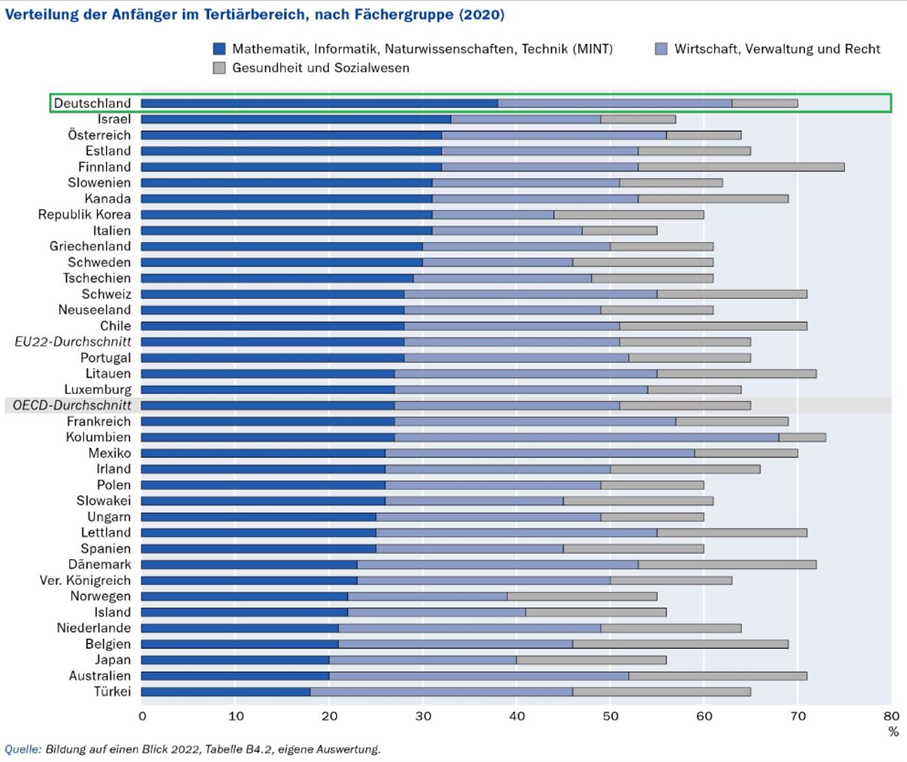
\includegraphics[width=0.95\textwidth]{terziaer}
	\caption{Anfänger im Tertiärbereich 2020 (\cite{BMBF.2022}, S. 1)}
	\label{fig:terziaer}
\end{figure*}

%nicht nur beim begeistern, sondern uach im Beruf
Bei den Frauen in technischen Berufen steht Deutschland mit seinem Anteil von knapp $17\,\%$ Frauen in technischen Berufen nur im Mittelfeld \cite{Honeypot.2018}. Besser stehen einige ehemalige Sowjetländer wie beispielsweise Bulgarien, anglophone Länder wie die USA, nordische Länder wie Finnland und einige muslimisch geprägte Länder wie der Iran und Malaysien (letztere zwei sind nicht in der Studie vertreten) da. \cite{Honeypot.2018} 

Schaut man sich die Frauen in technischen Berufen genauer an, zeigt sich eine Steigerung. So waren es im Jahr 2005 nur $205.000$ erwerbstätige Ingenieurinnen, in 2020 allerdings schon $312.900$.
Etwa jede dritte Ingenieurin findet den Weg in den Sekundärbereich, etwa ins Baugewerbe, in die Energie- und Wasserversorgung, die Elektroindustrie, den Fahrzeug- oder Maschinenbau. Die allermeisten Ingenieurinnen zieht es aber in den Tertiärbereich. Ein Fünftel von ihnen war zuletzt in der wissensintensiven Dienstleistung tätig, sie könnten etwa Forscherinnen sein. Rund $6\,\%$ der ausgebildeten Ingenieurinnen waren im Bereich Erziehung und Unterricht tätig. Hier werden auch die Grenzen der Aussagefähigkeit deutlich: Ob die ausgebildeten Ingenieurinnen tatsächlich in einem Ingenieurberuf oder als Managerinnen sowie Professorinnen mit ingenieurwissenschaftlichem Background arbeiten, bleibt unklar.

Auch internationale Vergleiche basieren auf Zahlen, die teilweise schwer vergleichbar sind. Beispielsweise ist der Gender Pay Gap in einem Land wie Rumänien niedrig, weil hier nur wenige Frauen in Arbeitsstatistiken erfasst werden, die dann aber vergleichsweise gut bezahlte Arbeit leisten.

\subsection{Historisch begründetes stereotypisches Bild eines deutschen Ingenieurs}
%warum
%STereotypisches Bild deutscher Ingenieur
% Vereinbarkeit beruf-Familie
Für Deutschland gilt abweichend von der allgemeinen Erläuterung von kulturellen Hemmnissen für Frauen im Technikfeld aus Abschnitt~\ref{sec:LernfaktorenBeiFrauen} eine historische Erläuterung. Denn als sich das Bild des deutschen Ingenieurs bildete, musste sich diese neue Berufsgruppe gegenüber den etablierten Handwerken und Naturwissenschaftlern erst behaupten. Auch in dieser Abgrenzung ist die Prägung des Mythos des deutschen Ingenieurs zu verstehen. Zu dieser Zeit aber, als die ingenieurwissenschaftliche Ausbildung an der Hochschule verortet wurde, waren Frauen dort als Studentinnen nicht zugelassen. 

Frauen, die heute in Deutschland ein ingenieurwissenschaftliches Studium wählen, brechen noch immer mit den Erwartungen, die ein Großteil der Gesellschaft an sie hat. Oft entwickeln sie deshalb Strategien wie ein Selbstbild als „untypische Frau“ um sich mit der Außensicht zu arrangieren.  

\subsection{Arbeitsmodelle der Ingenieure in Deutschland sind nur bedingt an Bedürfnisse der Frauen angepasst}
Hinzu kommt, dass gerade in der deutschen Industrie Ingenieure insbesondere in mittleren und großen Unternehmen gesucht werden, die ihre Jobs auf die Ernährerrolle ausgerichtet haben. Der Wandel hin zu einem Arbeitsmodell, dass die Vereinbarkeit Beruf und Familie in den Fokus nimmt, ist notwendig. Auch heute noch sind mehr Ingenieurinnen arbeitslos als Ingenieure. Dadurch zeigt sich, dass die vorherrschende Vorstellung, was der Ingenieurberuf verlangt, überwiegend auch stimmt. Andere Modelle wie beispielsweise Teilzeit nehmen aber zu und müssen von Role Models auch sichtbar gemacht werden (s. \ref{sec:Gespraechsprotokolle}.

%Auch Jette Hausotter sieht als zwei zentrale Gründe für Frauen, kein technisches Studium zu wählen, zum einen die Rollenwidersprüche zwischen der gesellschaftlichen Zuschreibung was weiblich ist und dem Berufsbild eines Ingenieurs/ einer Ingenieurin in unserer heutigen Gesellschaft zum anderen die als schwer vorstellbare Vereinbarkeit von Beruf und Familie für Ingenieurberufe. 
%\cite{Hausotter.2022} 
%nicht weg, hab ich nur woanders hingepackt (HB)

%Gleichberechtigungsparadox
%Gesellschaftlicher DRuck fehlt?

\subsection{Paradox der Gleichzeitigkeit von gegensätzlichem Anspruch und gelebter Realität}
%HB: Den folgenden Satz verstehe ich nicht
In der Forschung wird sich zudem mit dem Paradox der Gleichzeitigkeit von gegensätzlichem Anspruch und gelebter Realität klarkommen muss. (\cite{Weisenburger.07.03.2021}) Zudem wirkt hier ein Gleichberechtigungsparadoxon. Denn Länder wie Deutschland, die ein hohes Gleichberechtigungsideal haben, sind häufig nicht gleichzeitig die Länder in denen der Anteil von Ingenieurinnen besonders hoch oder der Gender Pay Gap besonders niedrig ist. 


%HB: Unklarer Satz für mih:
Prinzipiell gilt, dass eine kulturelle Veränderung viel Zeit in Anspruch nimmt und je nach Voraussetzungen unterschiedliche Ansätze und auch Ansprüche gelten. (vgl. \cite{Feder.2021} und \cite{}) 

Es gibt jedoch bei entsprechendem Druck und besonderen Situationen teilweise Fenster, um Änderungen schneller realisieren zu können. Ein Beispiel dafür ist die wirtschaftliche Krise in Spanien in den frühen 2010er Jahren, die dazu führte, dass Frauen, die studierten, zum größeren Anteil sichere und gut bezahlte Jobs in der Ingenieurbranche anstrebten. Auch in Deutschland kann es gerade ein solches Fenster in der Industrielandschaft geben, da durch die Produktionsstättenverlagerung weniger typische Ingenieurberufe in der Fertigung dafür aber zunehmend Stellen in der Entwicklung und dem Management besetzt werden. In diesen Rollen müssen sich Frauen weniger von Geschlechtsstereotypen abgrenzen, da organisieren und kommunizieren als weibliche Stärke gilt. 



%-------------------------------------
\section{Wer studiert zurzeit Elektrotechnik an der HTW Berlin?}
%-------------------------------------
\label{sec:StandBAETHTW}
%staatsangehörigkeit
%akademikerfamilie?

\subsection{Herkunft/ sozialer Satus}
In der Studienanfängerbefragung aus dem Sommersemester 2018 wurden Angaben zur sozialen Situation der Studierenden abgefragt. Daraus geht hervor, dass in der Elektrotechnik besonders wenige Frauen studieren ($11\,\%$). Ein Großteil der Studierenden der Elektrotechnik hat keine deutsche Staatszugehörigkeit (mind. $64\,\%$), nur $30\,\%$ von ihnen geben an Deutsch als Mutter- oder Erstsprache gelernt zu haben. Die Hochschulberechtigung haben $53\,\%$ der Studierenden im Ausland erworben, $32\,\%$ in Berlin, $0\,\%$ in Brandenburg und $15\,\%$ an anderen Orten in Deutschland. \footnote{Die Noten der Hochschulzugangsberechtigung lagen zur Hälfte zwischen $2,3$ und $3,0$, zu einem Drittel zwischen $1,6$ und $2,2$. Besonders gute Abschlüsse von $1,0$ bis $1,5$ bringen sieben Prozent und schlechte Noten von $3,1$ bis $4,0$ bringen elf Prozent mit.}


$61\,\%$ der Studierenden haben keinen familiären Akademiker-Hintergrund. 

Laut Sozialerhebung des Deutschen Studentenwerks sind $61\,\%$ der Bachelorstudierenden im Erststudium an HAWs während der Vorlesungszeit erwerbstätig. Für diese Jobs wenden sie durchschnittlich $13$~Stunden in der Woche auf \cite{Middendorf.2013}. (vgl. auch \ref{sec:ReissAuszuege})

Von den im Wintersemester 2022/23 immatrikulierten über $300$~Studierenden im Studiengang Elektrotechnik sind nur $36$~Frauen und davon haben nur acht einen typischen deutschen Namen. Genaue Daten über Migrationshintergrund werden nicht erhoben, nur über die Anzahl der ausländischen Studierenden. Die Zahlen zeigen, dass in den letzten Jahren die meisten Studentinnen im BA ET eine ausländische Hochschulzulassung haben.

\subsection{Passt das Niveau?}
Der überwiegende Teil der Studienanfänger*innen fühlt sich sehr gut oder gut auf das Studium vorbereitet ($77\,\%$). Damit fällt die Einschätzung in der Elektrotechnik trotz nicht deutlich besser Abschlussnoten positiver aus als in anderen Studiengängen des FB~1. Dies könnte kulturelle Hintergründe haben, da die Studienanfänger*innen in CE, RE und IKT deutlich seltener ihre Hochschulzugangsberechtigung im Ausland erhalten haben.
Auffällig ist, dass sich keine einzige weibliche Studienanfängerin sehr gut auf das Studium vorbereitet fühlt, während dies immerhin bei einem Fünftel der Studienanfänger der Fall ist. Dafür fühlen sich knapp $50\,\%$ der Studienanfängerinnen gut vorbereitet (Männer $40\,\%$), der Anzahl bei den Studienanfänger*innen kaum auf das Studium vorbereitet fühlt ist wiederum etwas höher bei den Frauen (Frauen: $19\,\%$, Männer: $13\,\%$). Diese Zahlen können nicht als analog zu den fachlichen Kompetenzen gesehen werden, weisen aber darauf hin, dass sich Frauen ihrer Voraussetzungen ein technisches Studium erfolgreich zu bewältigen unsicherer sind.

Immerhin ein Fünftel der Studierenden hat zuvor einen der folgenden Studiengänge abgebrochen: Medizin, Bauingenieurwesen, Computer Netzwerke, Design, Informatik, Sicherheitsmanagement, Ver\-an\-stal\-tungs\-technik und -management, Verkehrswesen und Wirtschaftsingenieurwesen. Außerdem haben $11\,\%$ zuvor eine der folgenden Berufsausbildungen abgeschlossen: Elektroniker*in, Fachkraft für Veranstaltungstechnik, IT-Assistent*in, Kaufmann/-frau im Groß- und Außenhandel, Kfz-Mechatroniker*in und Zerspanungsmechaniker*in. Dadurch fühlen sich über die Hälfte der Studienanfänger*innen mit Berufsausbildung sehr gut oder gut auf das Studium vorbereitet. Dies weist daraufhin, dass die Ausbildungsberufe als nah zu den Studieninhalten wahrgenommen werden. Auch fehlen bei den Berufsausbildungen der Studienanfänger*innen solche Exoten wie Koch/Köchin, Gärtner*in oder Augenoptiker*in wie in den Studiengängen CE, RE und IKT. 

Entsprechend zur Selbsteinschätzung der Studienanfänger*innen gut bis sehr gut auf das Studium vorbereitet zu sein nahmen in der ET am wenigsten Studienanfänger*innen am Brückenkurs Mathematik teil ($7\,\%$ teilweise, $12\,\%$ vollständig). Eine weitere Erklärung ist es, dass viele der Studienanfänger*innen bereits vor Aufnahme des Studiums arbeiten. Unter den Gründen warum der Brückenkurs nicht gewählt wurde, führt im FB~1 „Ich musste zu diesem Zeitpunkt arbeiten.“ ($28\,\%$). Darauf folgt „Ich wusste nicht, dass es den Brückenkurs gibt.“ ($24\,\%$) und erst dann „Ich habe gute Mathe-Vorkenntnisse.“ ($15\,\%$). 

\subsection{Motivation}
Entsprechend des vergleichsweise jungen Einstiegsalter der meisten Studierenden hat sich der Großteil bereits vor dem Abitur entschieden zu studieren ($73\,\%$). Dabei hat ein Drittel sich auch bereits für Elektrotechnik entschieden, während knapp $40\,\%$ erst bis ein Jahr nach der Schulzeit und $27\,\%$ sogar noch später sich für E-Technik entschieden hat.

Bei der Studienmotivation Elektrotechnik fällt auf, dass „Das Studium bietet Praxisorientierung“ bei den weiblichen Studierenden mit $60\,\%$ deutlich mehr genannt wird. Weitere wichtige Argumente für weibliche Studierende sind
\begin{itemize}
\item Weil mich Energie- und Automatisierungstechnik sehr interessiert
\item Das Studium verspricht vielseitige Berufsaussichten
\item Weil mir Mathe/Physik Spaß macht
\item Das Studium verspricht berufliche Sicherheit
\item Verwandte oder Freund*innen studieren bzw. studierten das Gleiche
\end{itemize}

Größtenteils sind die wichtigsten Gründe für Männer ähnlich nur der Grund berufliche Sicherheit ist für Frauen deutlich wichtiger. Am wenigsten wichtig sind für die befragten Frauen „die Arbeitsergebnisse anfassen zu können“, „aufgrund des Studiums in Deutschland leben zu können“, „der Ruf des Studiengangs“ sowie „die Möglichkeit im Studium persönliche Entfaltung/Kreativität“. Der häufigste Grund für Frauen den Studiengang Regenerative Energien zu studieren wurde nicht für ET abgefragt („Ich möchte die Welt verbessern.“). 

Gründe, die Studiengangs übergreifend für Studentinnen wichtiger waren als für Studenten, sind berufliche Sicherheit, vielseitige Berufsaussichten, Bekannte studier(t)en das Gleiche und Praxisorientierung.
Im Vergleich mit den anderen Studiengängen fällt des Weiteren auf, dass nur $22\,\%$ der ET-Studienanfänger*innen die möglichen Berufsfelder gut kennen. Je ein weiteres Drittel kennt die Berufsfelder eher oder kaum. Trotzdem sagen über die Hälfte, dass sie recht klare Vorstellungen von ihrem zukünftigen Beruf haben. 

\subsection{Zufriedenheit mit der Wahl des Studienfaches}
$28\,\%$ der Studienanfänger*innen sind sich sicher den richtigen Studiengang gewählt zu haben, für eine gute Hälfte trifft diese Aussage eher zu. Ein Fünftel ist sich eher unsicher. \cite{Rei.08.02.2019}


%\paragraph{Erwartete Probleme}


%Zusammmenfassung des Kaptels WEr studiert heute
\subsection{Zusammenfassung}

In den letzten Jahren hat sich das Bild der ET-Studierenden gewandelt. Zusätzlich zur allgemeinen Abnahme der Studienanfängerzahlen ist der Anteil Studierender mit ausländischer Hochschulzulassung stark gestiegen, während sich der Anteil von Frauen im Studiengang kaum verändert hat. Die Studierenden mit deutscher Hochschulzulassung kommen zumeist aus der Nähe der HTW Berlin. Frauen, die zurzeit ET studieren, nennen am häufigsten fachliches Interesse, Praxisorientierung, vielseitige und sichere Berufsaussichten sowie Bekannte mit derselben Studienerfahrung als Motivation für das ET-Studium. Die Frauen haben diverse Hintergründe. Sie kommen beispielsweise aus dem afrikanischen oder muslimisch-asiatischen Raum und weisen kulturell gesehen unterschiedliche DiSG-Profile auf (\cite{DeutschesInstitutfurMarketing.2022}. Frauen fürchten studiengangsübergreifend häufiger Probleme beim Kontakt zu Lehrenden zu bekommen. \cite{Rei.08.02.2019}

%-----------------------
\section{Welche Erfahrungen mit MINT-Frauenstudiengängen gibt es in Deutschland?}
%-----------------------
\label{sec:FSGinD}

Derzeit gibt es drei praktisch stattfindende MINT-Frauenstudienangebote in Deutschland. Einer davon ist der Frauenstudiengang Informatik und Wirtschaft an der HTW Berlin. Ein weiterer Informatik-Studiengang wird in Bremen angeboten. Der dritte Studiengang ist im Bereich Maschinenbau an der Hochschule Ruhr-West.
Andere Frauenstudienangebote wurden bereits wieder eingestellt oder pausieren (siehe Abb.~\ref{tab:mintFSG}). Die Gründe sind zumeist sinkende Bewerberzahlen, deren Gründe allerdings nicht im einzelnen nachvollziehbar sind. 


\begin{figure*}[!bt]
\centering
\begin{tabular}{ |p{3.0cm}||p{4.5cm}|p{3.5cm}|p{5cm}|  }
 %\hline
 %\multicolumn{4}{|c|}{MINT-Frauenstudiengänge in Deutschland} \\
 \hline
 Hochschule                     & Studiengang   & Jahr des Angebots  & Entwicklung der Studienanfängerinnen\\
 \hline
 \hline
 Jade Hochschule Wil\-helms\-ha\-ven  & Wirtschafts\-inge\-ni\-eurwesen  & ab 1997 einige Jahre lang &   zu wenige\\\hline
Hochschule Bremen               & Internationaler Frauenstudiengang Informatik  & seit 2000   & besteht weiterhin\\\hline
 Hochschule Furt\-wang\-en      & WirtschaftsNetze/ eBusi\-ness (Inf/ Wirt) & 2002-2020 & zu wenige - auch aufgrund von Wechsel zu zentraler Studienplatzvergabe in Ba-Wü (zuvor $90$~Stud.anf. pro Jahr)\\\hline
 Hochschule Stralsund           & Wirtschafts\-inge\-ni\-eurwesen & einige Jahre lang & zu wenige\\\hline
 Ernst-Abbe-Hoch\-schule Jena   & Elektro- und Informationstechnik  & seit 2015 & wurde in diesem Semester kaum nachgefragt\\\hline
 Hochschule Ruhr-West& Maschinenbau  & seit 2018   & wurde in diesem Semester kaum nachgefragt\\\hline
 HTW Berlin & Informatik und Wirtschaft  & seit 2009 & besteht weiterhin mit hoher Nachfrage\\
 \hline
\end{tabular}
\caption{Zusammenfassung MINT-Frauenstudiengänge in Deutschland, Quellen: \cite{Degener.25.03.2021}\cite{Weidner.2022}}
\label{tab:mintFSG}
\end{figure*}


Generell gilt, dass mit diesen Studiengängen spezielle Gruppen von Frauen angesprochen werden sollen, die in der Regel nicht selbst aktiv auf der Suche nach MINT-Studienangeboten sind. Aus diesem Grund steht und fällt der Erfolg eines guten Studienangebotes mit der Sichtbarkeit des Angebotes. So gab der Dekan Prof. Jack der EAH Jena an, dass das Angebot seiner Hochschule während der drei Jahre, die es von einer Projektmitarbeiterin begleitet und beworben wurde, deutlich besser angenommen wurde als in den letzten Jahren. Auch Prof. Dorschu von der Hochschule Ruhr-West gibt im persönlichen Gespräch an, dass die Bewerberzahlen zurück gegangen sind als sie keine Infoveranstaltungen in Präsenz machen konnten. 

Hinzu kommt, dass einige Frauenstudiengängen an eher unattraktiven Studienorten begründet wurden um Bewerberinnen an ihre Hochschule zu holen. Die erfolgreichen Studiengänge für Informatik befinden sich dahingegen in den Stadtstaaten Bremen und Berlin.





%-----------------
\section{Welche Zielgruppe soll ein Frauenstudiengang „Elektrotechnik und Gesellschaft“ ansprechen?}
%-----------------------
\label{sec:unsereZielgruppe}

%Zusammenfassung: andere Frauen als bisher, die den geschützen Raum suchen oder brauchen
%Locken mit coolem Titel politische Inhalte


%andere Frauen als bisher: (die vorher Angst hateen, sich nicht trauten, keine bock auf Nerds hatten
%Quereinsteigerinnen die keine Angst mehr haben vor den Inhalten
%Vereinbarkeit von Beruf+ Familie
%Frauen mit Migrationshintergrund

%geschützer Raum (=monoeduktativ)
%mit gleichgesinnten
%positive disktriminierung

%\subsection{Frauen, die bisher Elektrotechnik nicht studieren wollten}

In qualitativen Interviews mit den Dekanen und Studiengangsleiter*innen ähnlicher, monoedukativer Angebote wurde für jedes dieser Angebote festgestellt, dass sich Frauen immatrikulierten, die ohne das mono-edukative Angebot nicht dieselbe technische Fachrichtung gewählt hätten. (vgl. \ref{sec:Gespraechsprotokolle}) 


\subsection{Quereinsteigerinnen?}

\subsection{Frauen, die etwas sinnvolles studieren wollen}
Die besondere Attraktivität des FIW hat zu einem Drittel der Studierendenanzahl auch mit Quereinsteigerinnen zu tun, die bereits älter und berufstätig sind und sich nun mit Informatik-Fähigkeiten weitere Karrierewege vor dem Hintergrund ihrer ursprünglichen (Aus-)Bildung zu erschließen. Letztere Kategorie würden wir mit unserem Angebot eher nicht erreichen. Allerdings ist eine Attraktivität für junge Frauen, die etwas Sinnvolles studieren wollen weiterhin gegeben. Anders als in der Informatik bleibt es in der Elektrotechnik allerdings unumstößlich wichtig eine Nähe zur Mathematik mitzubringen.

\subsection{Frauen mit Migrationshintergrund }
Frauen mit Migrationshintergrund werden bereits im derzeitigen Elektro\-tech\-nik-Studium erreicht. Allerdings gibt es bereits Hinweise von Lehrenden, dass Einzelne von ihnen in einer reinen Frauen-Gruppe unbedarfter lernen könnten über die Inhalte zu diskutieren und Fragen zu stellen. 

\subsection{Frauen, die einen geschützten Raum suchen}
%HB: Monoedukativer Unterricht bietet einen geschützen Raum und senkt kulturelle Hemnisse

%HB: Der folgende Absatz ist für mich nicht sehr überzeugend.. Zeigt OJA nicht eher, das Frauen auf Vielfältigkeit abfahren?
Auch in einem weiteren Format, das für MINT-Förderung ins Leben gerufen wurde, konnte dies beobachtet werden. Im O ja! werden - ohne das dies beabsichtigt war - bereits vergleichsweise mehr weibliche MINT-Interessierte erreicht, als in anderen MINT Ausbildungen und Studiengängen. Dies gilt sowohl für Studentinnen mit deutscher als auch mit ausländischer Hochschulzulassung.
Geplante monoedukative Empower-MINT Formate für Frauen wurden allerdings nicht oder nur vereinzelnd wahrgenommen. Als Argument wurde häufig angeführt, dass sie nicht gesondert behandelt werden wollen (vgl. \emph{Othering}). Dies weist darauf hin, dass einzelne Angebote, die nach Geschlecht trennen unangenehm den Unterschied zwischen Männern und Frauen betonen. Ist die monoedukative Phase allerdings in sich abgeschlossen, erleben Studentinnen stärker den Zusammenhalt in der Gruppe.

Studentinnen mit nicht-deutscher Hochschulzulassung kommen meist aus akademischen und bereits technisch geprägten Haushalten. Sie haben die entsprechende Unterstützung aus dem Elternhaus eine Ingenieurinnenkarriere anzugehen. Trotzdem meinen sie eine Vergewisserung ihrer Fähigkeiten durch ein MINT-Orientierungsjahr zu benötigen.
Es gab und gibt wahrscheinlich Teilnehmerinnen, die sich in einem monoedukativen Rahmen ggf. anders gezeigt und Fragen gestellt hätten. Eine ehemalige Teilnehmerin mit nicht-deutscher Hochschulberechtigung studiert nun den Frauenstudiengang Informatik und Wirtschaft und entwickelt sich dort sehr gut. Sie findet es befremdlich, dass dies ein reiner Frauenstudiengang ist und somit nicht die Realität in der Arbeitsweit abbildet. Auf Nachhaken stimmt sie allerdings zu, dass sie nun im Studiengang mehr eigene Fragen stellt. (Anmerkung: das könnte aber auch mit online vs. Präsenz zu tun haben. Sie startete das O ja! im April 2020.)

Auch in vielen anderen Gesprächen mit Frauen, die sich bereits in der bestehenden MINT-Bildung und -Arbeitsmarkt bewegen, kam nach einer zunächst bestehenden Ablehnung eine Einsicht, dass positive Diskriminierung Frauen voranbringen kann. Ein Beispiel:
\emph{"People want to be recognized for their capabilities, she says, so women don’t want to be hired based on their gender. “But I decided not to let that stop me. The further I got in my career, the fewer women I saw. So although I am ambivalent about discriminating against men, we need to do this now, and hopefully it will later sustain itself." \cite{Feder.2021}}

%allerdings ist auch heute noch der Gender Pay Gap in der Industrie.

\subsection{Frauen, die den Standortvorteil Berlin schätzen}
%HB: Hm, passt das hierher?
Abb.~\ref{fig:DataMINT} zeigt, dass im  Deutschlandweiten Vergleich der Anteil an Frauen in den MINT-Studienfächern nach einem Peak in 2015 in Berlin weniger stark zurück gegangen ist  als in anderen Bundesländern. Dies kann mit der Attraktivität des Hochschulstandortes Berlin zusammenhängen.

%hier nebeneinander die DataLabMint-Bilder!!!
\begin{figure}[!ht]
	\centering
\psfrag{m}[cc][cc]{$m$}
	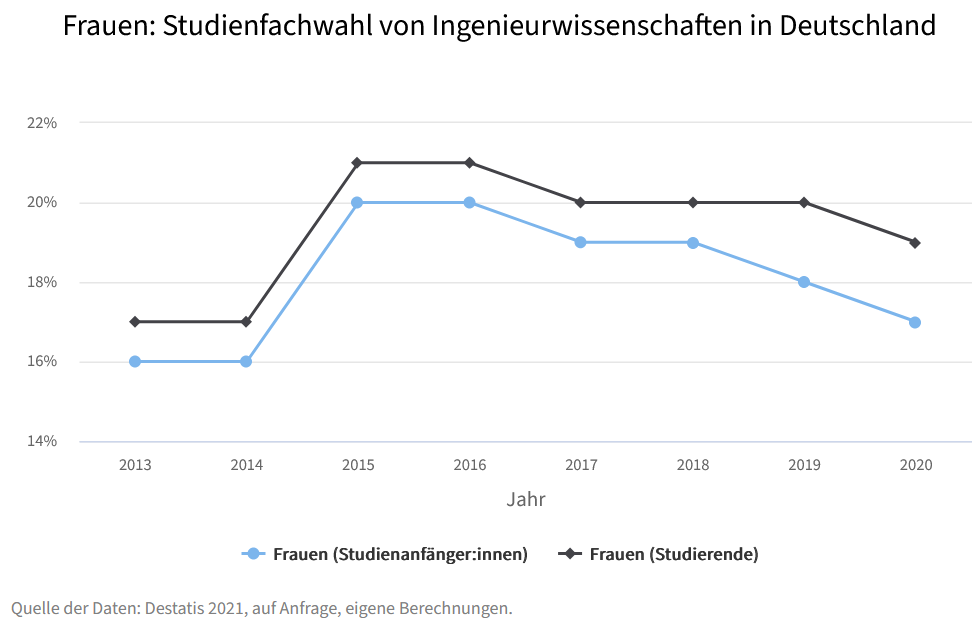
\includegraphics[width=0.95\columnwidth]{DataLabMINT_Frauen Ing 2013 bis 2020.png}
    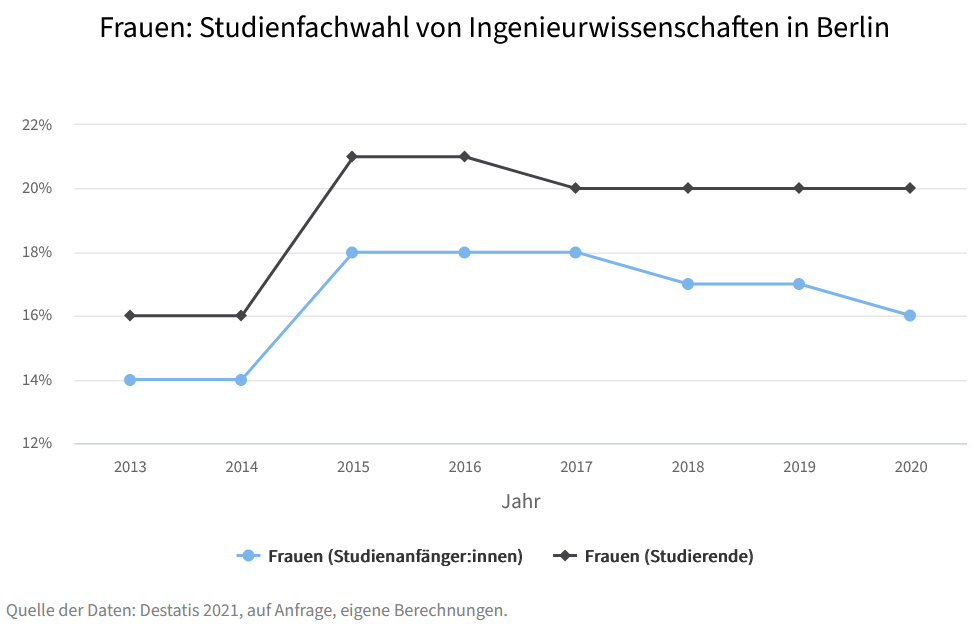
\includegraphics[width=0.95\columnwidth]{DataLabMINT_Frauen Ing 2013 bis 2020_Berlin.png}
	\caption{Entwicklung der Anzahl von Studienanfängerinnen und Studentinnen in Ingenieursstudiengängen an Hochschulen in Deutschland und Berlin \cite{MINTvernetzt.17.01.2023}.}
	\label{fig:DataMINT}
\end{figure}

\subsection{Frauen, die (dank neuer Lehrformen und -inhalte) auch gesellschaftspolitische Themen im Rahmen des Elektrotechnikstudiums behandelt wissen}
%HB: weiß nicht, ob das hier sinnvoll ist, aber irgdwie ist das ja auch Zielgruppe...

\subsection{Frauen, deren Zweifel am Berufsbild Elektrotechnikingenieur aufgrund eines guten Marktetings und eines tollen Studiengang- Namens verfliegen}
%HB: weiß nicht, ob das hier sinnvoll ist, aber irgdwie ist das ja auch Zielgruppe...
%------------------------------
\section{Fazit}
\label{sec:Fazit}
%-------------------------------
Ein Frauenstudiengang einzurichten und erfolgreich zu betreiben, ist kein Selbstläufer. Gerade im unattraktiven Berufsfeld Elektrotechnik reicht es nicht ein diverses, gesellschaftspolitisch relevantes Studium zu organisieren. Es gehört auch ein umfassendes Marketing dazu, um potenziellen Studentinnen aufzuzeigen wie sie ihre MINT-Fähigkeiten einsetzen können, um nach einem interessanten und relevanten Studium in einen lebenswerten Beruf zu starten. Auch Unternehmen aus der Branche müssen sich für diese Kommunikationsleistung einbringen. Eine aktive Begleitung der verschiedenen Maßnahmen um ein Elektrotechnik-Studium für Frauen attraktiv zu machen, ist nötig. 

Positiv stimmen kann die Erkenntnis, dass es viele Frauen mit guten MINT-Fähigkeiten gibt, die für ein Elektrotechnik-Studienangebot gewonnen werden können.


%\newpage
\bibliography{FSG}

%\newpage
%-------------------------------------
\section{Anhang}
%-------------------------------------

\subsection{Auszüge aus: Ergebnisse der Studienanfänger\-befra\-gung \cite{Rei.08.02.2019}}\label{sec:ReissAuszuege}

\subsubsection*{2.1.1 Frauenanteil (S. 3)}

Prinzipiell gilt, dass erst ein Anteil von $30$~Prozent einer Minderheit ermöglichen, anders wahrgenommen zu werden und als Gruppe Veränderungen herbeizuführen. 
\footnote{„Komm, mach MINT.“ Nationaler Pakt für Frauen in MINT-Berufen: MINT-Fächer stark nachgefragt. Pressemitteilung vom 19.12.2016. \url{http://www.komm-mach-mint.de/Presse/Pressemitteilungen/ MINT-Faecher-stark-nachgefragt.}}
Auch im Studiengang Regenerative Energien liegt der Frauenanteil unter diesem Wert. Die vorherrschenden Geschlechtsstereotype und der niedrige Frauenanteil dieser Fächer könnten sowohl auf potentielle
Studienbewerberinnen abschreckend wirken als auch für Studentinnen besondere Hürden im Studium mit sich bringen.

\subsubsection*{3.1. Studentinnen am Fachbereich I}
Die Frauenanteile der untersuchten Studiengänge mit Ausnahme des Studiengangs IKT sind sehr niedrig (vgl. Kapitel 2.1.1 auf Seite $3$) und können ggf. durch ein gendersensitives Hochschulmarketing und weitere Maßnahmen erhöht werden. Es stellt sich die Frage, wie sich die niedrigen Frauenanteile in den genannten Studiengängen auswirken und ob Studentinnen besondere Hürden
im (männerdominierten) Studium erleben.

Bei den Selbsteinschätzungen und Befürchtungen hinsichtlich des Studiums zeigt sich innerhalb der Gruppe der Frauen kein einheitliches Bild. Bei der Frage, wie gut sich die Studienanfänger*innen durch die Schule auf das Studium vorbereitet fühlen, schätzen sich Frauen deutlich schlechter ein als Männer. Keine einzige fühlt sich „sehr gut“ vorbereitet, während dies auf 19\% der Männer zutrifft (vgl. Abbildung 2.13 auf Seite 13). Im Studiengang IKT mit dem höchsten Frauenanteil äußern Frauen deutlich häufiger als Männer.

Befürchtungen hinsichtlich der sozialen Integration ins Studium (Kontakte zu anderen Studierenden (Abb.~2.36 auf Seite~$32$) und zu Lehrenden (Abb.~2.39 auf Seite~$35$). Zugleich befürchten sie seltener Leistungsprobleme als Männer in diesem Studiengang (z.B. hinsichtlich Prüfungsversagen (Abb.~2.42 auf Seite~$39$) oder Leistungsproblemen (Abb.~2.43 auf Seite~$40$)). Insgesamt fällt auf, dass Frauen häufiger als ihre männlichen Kommilitonen an der Wahl des Studiengangs zweifeln (vgl. Abb.~2.45 auf Seite~$42$). Zu berücksichtigen ist hierbei, dass es sich um die Wahrnehmung zu Studienbeginn, handelt, die sich im Studienverlauf ändern kann.

Die Frage der Vereinbarkeit von Familie und Studium scheint zum Zeitpunkt des Studienbeginns nur für wenige Studierende ein Problem zu sein und wenn doch, dann stellen sich Frauen und Männer diese Frage gleichermaßen (vgl. Abb.~$2.38$ auf Seite~$34$).

\subsection{Gesprächsprotokolle über Erfahrungen mit MINT- Frauenstudiengängen}\label{sec:Gespraechsprotokolle}

\subsubsection{Ernst-Abbe-Hochschule Jena}
FG ET/IT an der EAH Jena - getrennte Studieneingangsphase im Übungs- und Praktikumsbetrieb defacto wird dies zurzeit nicht mehr durchgeführt, monoedukative Eingangsphase war angedacht, wurde aber nicht gut angenommen, wahrscheinlich da die Studierenden nicht ge"othert" werden wollten

Übungs- und Praktikumsbetrieb, nicht für die Vorlesung; getrennte Studieneingangsphase, in den ersten drei Jahrgängen (ab WiSe 2015/16) halbwegs gut gelaufen, Bewerberinnen waren zufrieden, aber dann nur noch zwei bis drei Studentinnen, im aktuellen Jahrgang keine Anmeldung; $2,5$~Jahre gab es Projektmitarbeiterin, die agil war und durch Werbung und Öffentlichkeitsarbeit zum Erfolg beigetragen; Anteil Studentinnen konstant bei zwischen $17\,\%$ und $20\,\%$; vor der Maßnahme war er bei $7--10\,\%$; die Workshops vor Beginn der ET-FSG waren teilweise Gendersensibilisierung, aber auch Verhalten/ Ansprache; Maßnahme begleitet durch Interviews; Studentinnen fanden eigene Gruppe zum Ausprobieren in der Eingangsphase gut, aber wollten auf keinen Fall andere Behandlung/ Themen; geringere Abbrecherquote unter Frauen; aus dem Frauenstudiengangsangebot haben alle den Abschluss geschafft; im ersten Jahr gab es durch Projektmitarbeiterin, SHKs und Absolventinnen regelmäßige Mentoring-Treffen, ab dem zweiten Jahr haben die älteren Studentinnen Mentoring für die Studienanfängerinnen gemacht, selbst organisiert Treffen mit Absolventinnen; ggf. weiterhin hoher Frauenanteil weil absolute Zahlen gesunken sind? zurzeit sieben bis acht Frauen unter $40$~Studierenden in der ET; damals rund $50$~Studierende; extremer Widerstand an der Hochschule unter den Dozierenden, deswegen kein FSG, sondern nur Übungsangebot in der Studieneingangsphase
[Telefonat mit Dekan Prof. Oliver Jack; 22.11.2022 von 10.30-11 Uhr]

\subsubsection{Hochschule Ruhr West in Mülheim an der Ruhr}
Frauenstudiengang Maschinenbau - geführt als eigenständiger Studiengang, ist formal aber eine Studiengangsvariante mit denselben Inhalten und teils identischen Prüfungen wie der gemischte Maschinenbau-SG. Im sogenannten Y-Modell studieren Frauen seit dem WS 2018 die ersten vier Semester monoedukativ und studieren danach koedukativ bis zum Ende.

Ein Vorteil dieser Variante ist, dass die Frauen, die gemischt studieren wollen das weiterhin tun können. Außerdem kann die Chancengleichheit für Männer durch die identischen Modulhandbücher gewährleistet werden. Auch ist die Entscheidung für ein identisches Curriculum strategisch getroffen worden, um dem Vorwurf des \emph{Studium light} zu begegnen.

Frau Prof. Dorschu kann für ihren SG bestätigen, dass sie Studentinnen erreicht, sonst nicht Maschinenbau studiert hätten. Sie wollten vorurteilsfrei studieren und sich - zumindest anfangs - nicht für ihr geschlechtuntypisches Studium rechtfertigen müssen. Generell gilt für $90\,\%$ der Studierenden im Maschinenbau, dass sie einen persönlichen Zugang aufgrund eines Verwandten mit Maschinenbau-Ingenieurabschluss haben.

Laut Prof. Dorschu sei der Wechsel ins gemischte Studium ab dem fünften Semester gut verlaufen. Die Studentinnen fühlten sich gut ausgebildet, selbstbewusst, offen und ein Rückfall in alte Muster von Unsicherheit sei nicht zu beobachten.

Eine Mischung der Studierenden in den ersten Semestern ist nicht vorgesehen. Die Studiengangsleitung verhindert "Modultourismus", wenn jemand beispielsweise lieber bei einer anderen Dozierenden das Modul hören möchte. Projektarbeit wird allerdings interdisziplinär geleistet und dies sei auch wertvoll um Vorurteile gegenüber dem Frauenstudiengang abzubauen.

Zuletzt war es interessant zu hören, dass das nordrhein-westfälische Bildungsministerium zunächst gegen den Frauenstudiengang war. Sie ließen sich aber insbesondere mit dem Argument überzeugen, dass für Männer ein gleichwertiges Studium angeboten würde. Die nun zuständige Mitarbeiterin des Ministeriums sei sogar "Fan" des Angebots.
[Videokonferenz mit Prof. Dorschu, Studiengangsleiterin Frauenstudiengang Maschinenbau und Prof. Brandtstädter; 07.12.2022]

\subsubsection{Zentrales Referat für Frauenförderung \& Gleichstellung, HTW Berlin}
Für Deutschland gilt abweichend von der allgemeinen Erläuterung von kulturellen Hemmnissen für Frauen im Technikfeld aus Abschnitt~\ref{sec:LernfaktorenBeiFrauen} eine historische Erläuterung. Denn als sich das Bild des deutschen Ingenieurs bildete musste sich diese neue Berufsgruppe gegenüber den etablierten Handwerken und Naturwissenschaftlern erst behaupten. Auch in dieser Abgrenzung ist die Prägung des Mythos des deutschen Ingenieurs zu verstehen. Zu dieser Zeit aber als die ingenieurwissenschaftliche Ausbildung an der Hochschule verortet wurde, waren Frauen dort als Studentinnen nicht zugelassen. 

Frauen, die heute ein ingenieurwissenschaftliches Studium wählen, brechen noch immer mit den Erwartungen, die ein Großteil der Gesellschaft an sie hat. Oft entwickeln sie deshalb Strategien wie ein Selbstbild als „untypische Frau“ um sich mit der Außensicht zu arrangieren.  
Hinzu kommt, dass gerade in der deutschen Industrie Ingenieure insbesondere in mittleren und großen Unternehmen gesucht werden, die ihre Jobs auf die Ernährerrolle ausgerichtet haben. Der Wandel hin zu einem Arbeitsmodell, dass die Vereinbarkeit Beruf und Familie in den Fokus nimmt, ist notwendig. Auch heute noch sind mehr Ingenieurinnen arbeitslos als Ingenieure. Dadurch zeigt sich, dass die vorherrschende Vorstellung, was der Ingenieurberuf verlangt, überwiegend auch stimmt. Andere Modelle wie beispielsweise Teilzeit nehmen aber zu und müssen von Role Models auch sichtbar gemacht werden.
[Telefonat mit Dr. Jette Hausotter; 11.01.2023]

\end{document}
